\section{Exeperiments and Results}
\label{sec:benchmark}

In this section, we demonstrate the efficacy of our approaches via a set of benchmarks.

\subsection{Experiment setup}

Wne carried our experiments on Mira, a Blue Gene/Q supercomputer. In our experiments, we varied paritition size from 512 nodes up to 8012 nodes. The experiments involved a subset or entire set of nodes for each partition. The number sources and destinations and the distance between them are also varied depending on each experiment. We also varied the number of ranks from 1 rank per node up to 8 ranks per node to show the efficacy of our work if multiple ranks per node are used. Data size to be exchanged is also varied from 512 KB up to 8 MB per pair of communication. Our experiments covered 3 communication patterns: disjoint, overlap and subset. For the commnication patterns, we demonstrated the efficacy of our algorithms in comparions with MPI\_Alltoallv.

\subsection{MPI Paths Reconstruction}

In our experiment, we need to measure not only the performance of MPI routines but also loads on physical links and number of hops of path that MPI takes to move data from a set of sources to a set of destination. The load and hops informaiton can reveal insight of performance difference between MPI and our framework OPTIQ. Thus reconstructing MPI's paths is necessary to get load and hops information.

We reconstruct MPI's paths based on our understanding of default routing algorithms described in \cite{Chen:BGQ}. For each pair of source and destination, we start at a source node and follow the rules of the routing algorithm to move data from the source node to its destination. We then record paths for all the pairs and use them to calculate load and number of hops. 

\subsection{Communication Patterns}
In this paper we demostrate data movement performance of our OPTIQ framework and existing MPI's routines on the following communication patters:

\begin{figure}[ht]
\vspace{-0.1in}
\centering
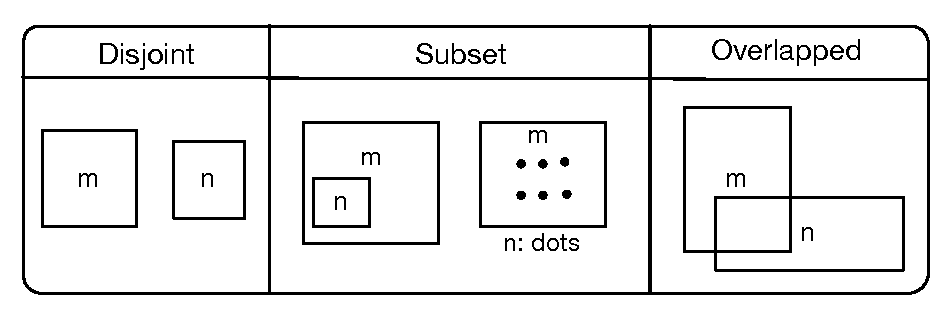
\includegraphics[scale=0.55]{figures/patterns.pdf}
\vspace{-0.1in}
\caption{Communication patterns}
\vspace{-0.1in}
\label{fig:patterns}
\end{figure}

\begin{itemize}
\item Subgroup Data Aggregation: a special case of All to many (or many to many.)
\item Many to many: disjoint sets.
\item Many to many: overlapped sets.
\item Many to many: subsets. In this category, there are 2 sub types: (Type 1) concetrated subset of destinations and (Type 2) distributed destination nodes as in I/O data aggregation.
\end{itemize}

We carried a set of experiments to study the system's behavior in various patterns and demontrate throughput improvement.

\subsection{Experimental results}

In the experiments, we collected the throughput and loading related information while varying communication patterns, partition sizes, message sizes, number of MPI ranks per node.
In the next subsections, we go into each communication and study in details the system's behaviors and performance.

The number of sources: m, number of destination n, ratio between m and n is r, total number of node is p, average distance between sources and destinations is d

Explain about what were being measured: hopbytes. Explain about the 90 tests we did and the avereage improvements.

\begin{figure*}[!htbp]
        \centering
        \begin{subfigure}[b]{0.32\textwidth}
                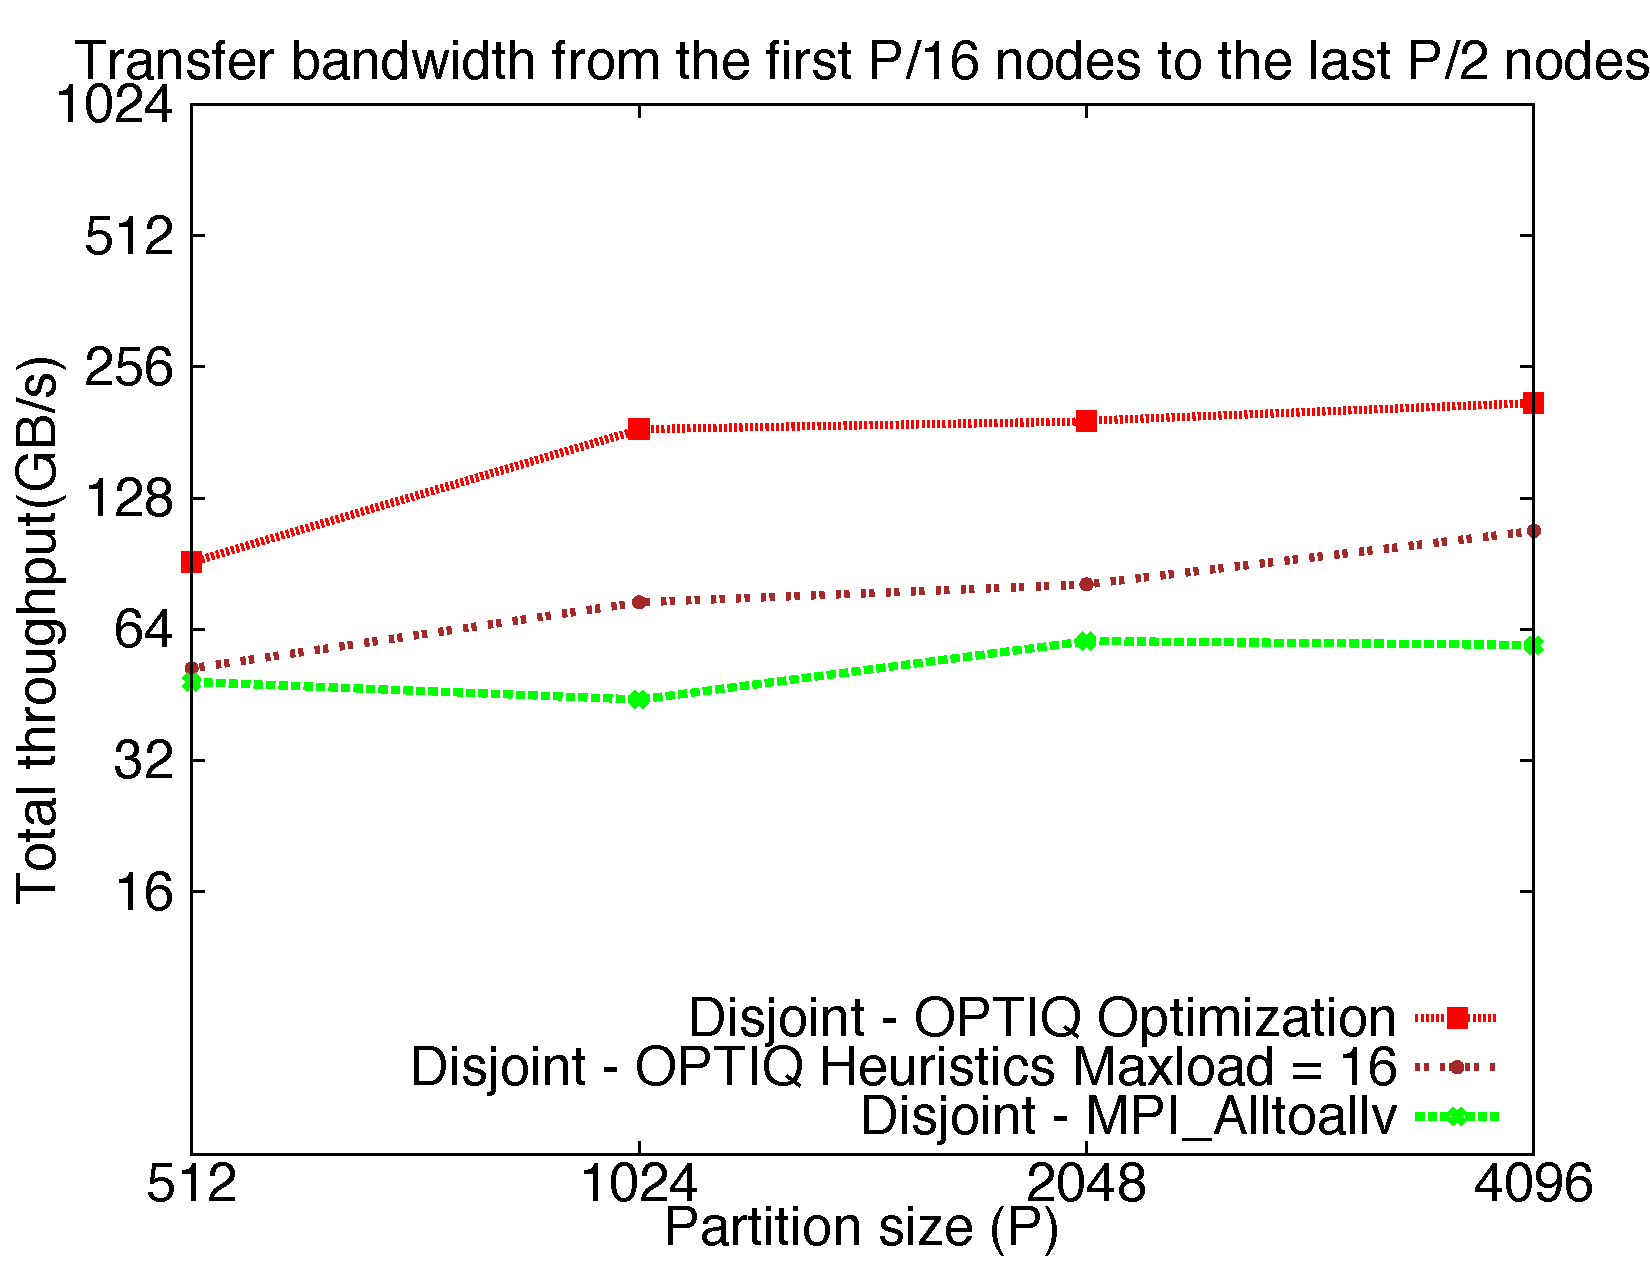
\includegraphics[width=\textwidth]{figures/constantr_3.pdf}
                \caption{Disjoint}
                \label{fig:3_1024_hop}
        \end{subfigure}%
        ~ %add desired spacing between images, e. g. ~, \quad, \qquad, \hfill etc.
          %(or a blank line to force the subfigure onto a new line)
        \begin{subfigure}[b]{0.32\textwidth}
                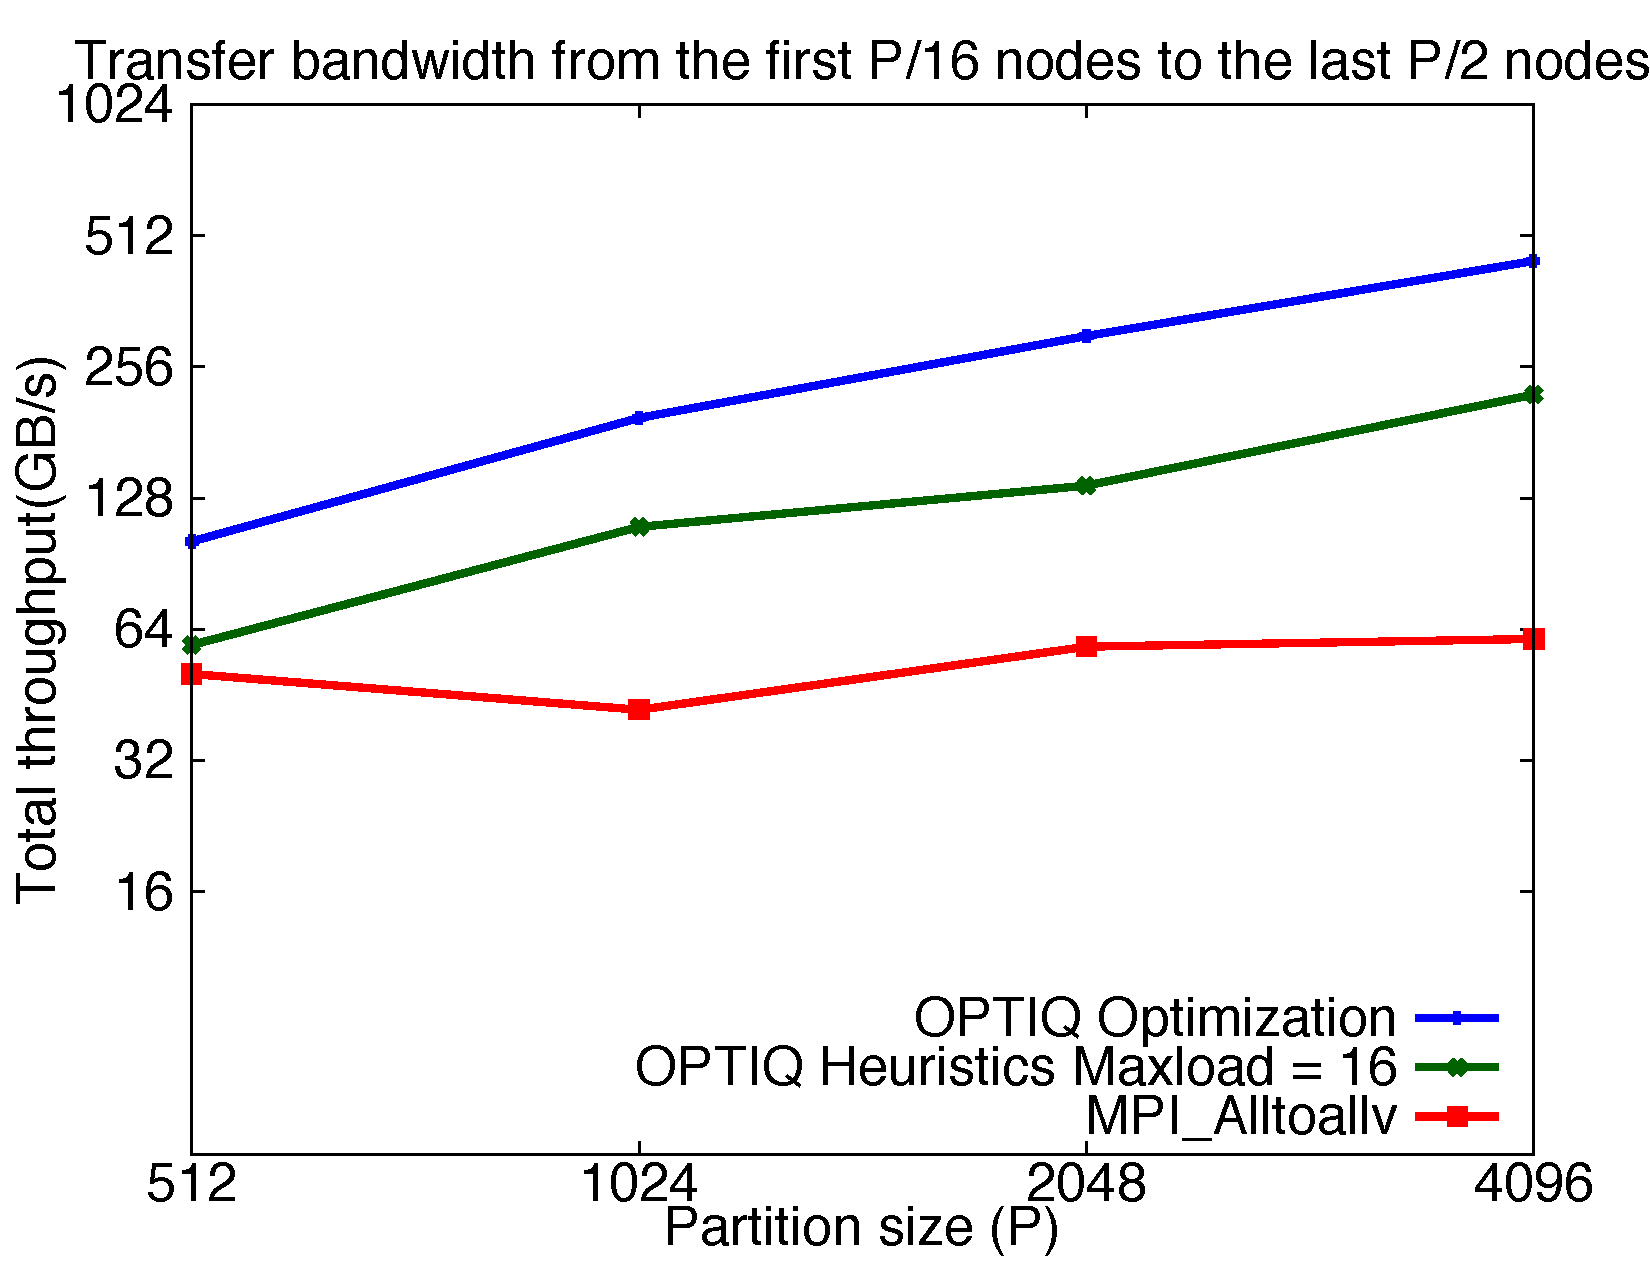
\includegraphics[width=\textwidth]{figures/constantr_27}
                \caption{Overlap}
                \label{fig:3_1024_hopbyte}
        \end{subfigure}
        ~ %add desired spacing between images, e. g. ~, \quad, \qquad, \hfill etc.
          %(or a blank line to force the subfigure onto a new line)
        \begin{subfigure}[b]{0.32\textwidth}
                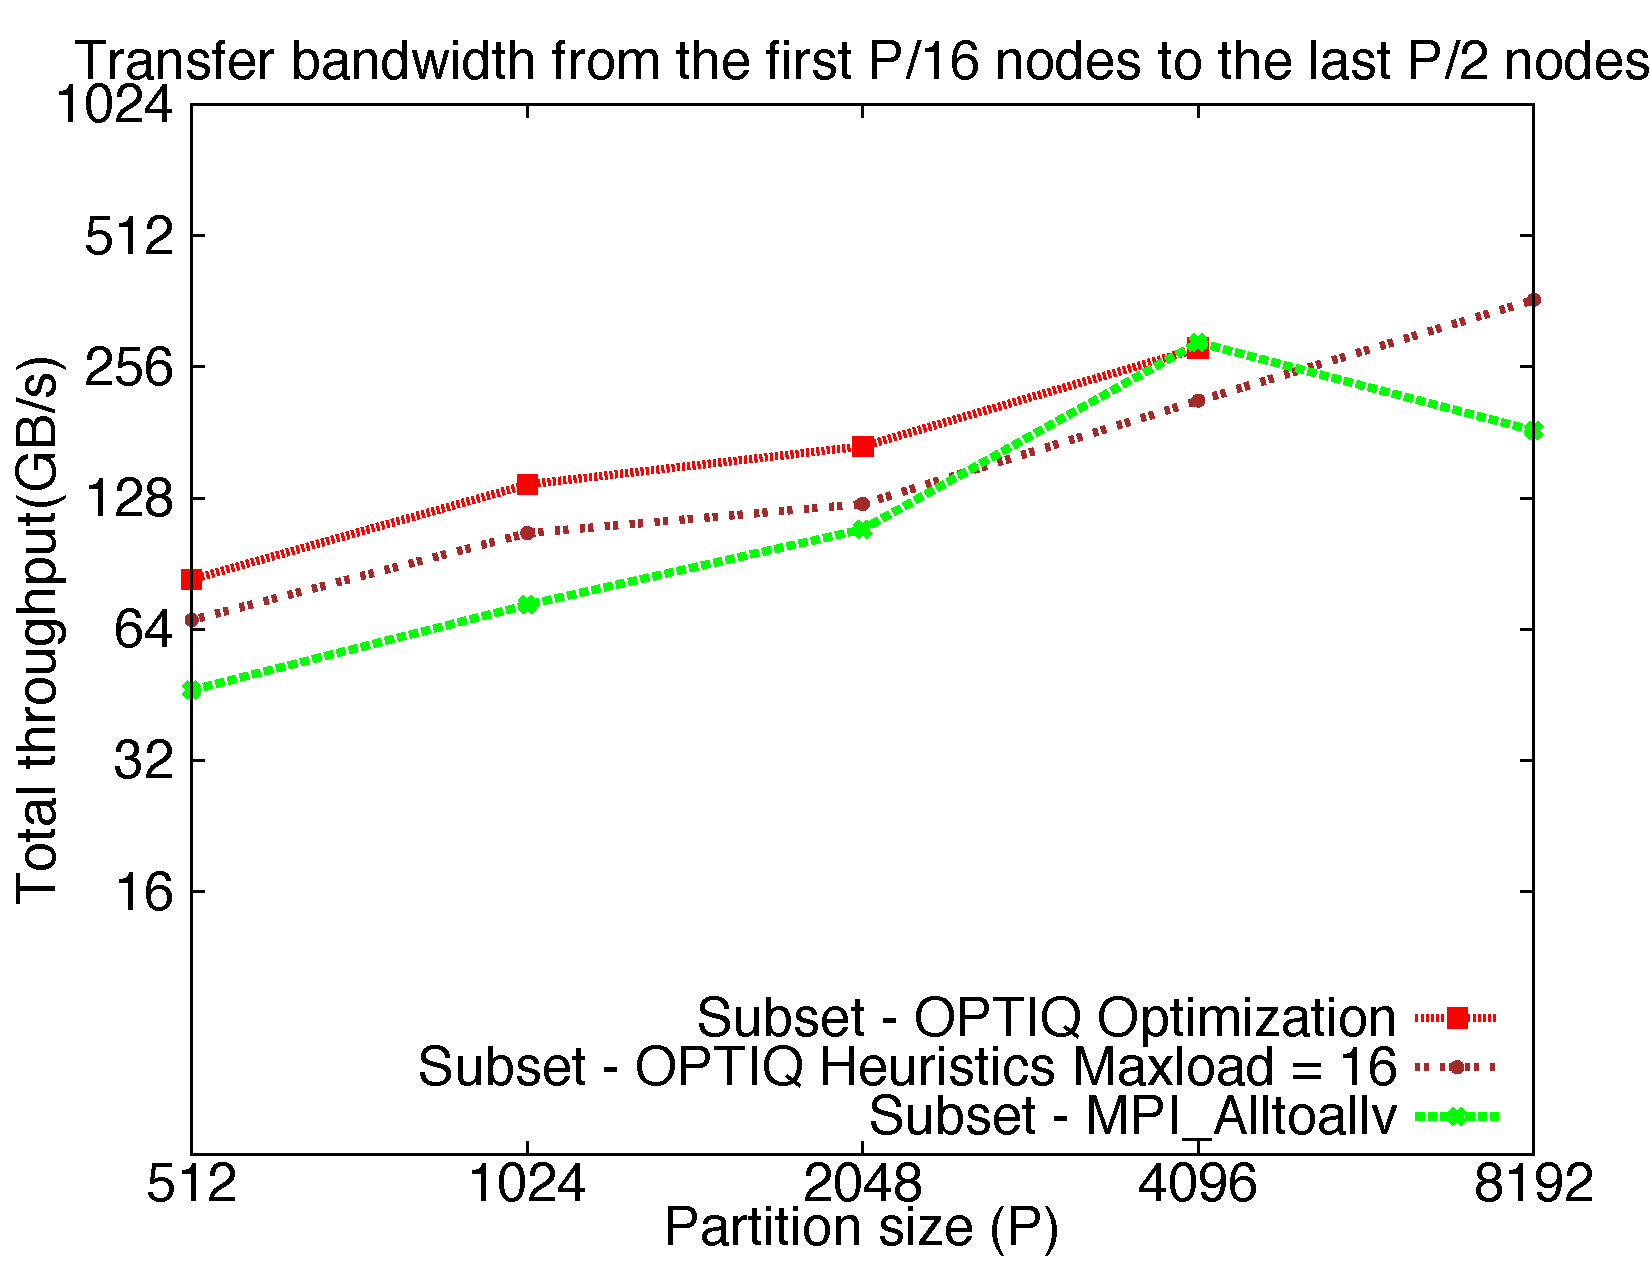
\includegraphics[width=\textwidth]{figures/constantr_87}
                \caption{Subset}
                \label{fig:3_1024_hopcopy}
        \end{subfigure}
        \caption{Varying the number of sources and destinations and total number of nodes while keeping the ratio constant (1:8) }
        \label{fig:3_1024_histo}
\end{figure*}

\begin{table*}[!htbp]
   \centering
    \begin{tabular}{| l | l | r | r | p{0.5cm} | p{0.5cm} | p{0.75cm} | p{0.75cm} |p{0.5cm} | p{0.5cm} |p{0.5cm} | p{0.5cm} |p{0.75cm} | p{0.75cm} |}
    \hline
    \multirow{3}{*}{Pattern} & \multirow{3}{*}{Type} & \multirow{3}{1cm}{BW (GB/s)} & \multicolumn{3}{ c| }{Num. of Paths} & \multicolumn{2}{ c| }{Hopbytes} & \multicolumn{2}{ c| }{Num of copies}& \multicolumn{2}{ c| }{Num of paths} & \multicolumn{2}{ c| }{Total data} \\ \cline{4-6}
    & & & \multirow{2}{0.5cm}{Total Paths} & \multicolumn{2}{ c| }{Per Job} & \multicolumn{2}{ c| }{Per Path (MB)} & \multicolumn{2}{ c| }{Per Path}& \multicolumn{2}{ c| }{Per Link}& \multicolumn{2}{ c| }{Per Link (MB)} \\ \cline{5-14}
    & & & & {Max} & Avg & Max & Avg & Max & Avg & Max & Avg & Max & Avg\\ \hline
    \multirow{3}{*}{Disjont} & OPT    & 188.62 & 1,169 & 6 & 2.28 & 83.88 & 23.02 & 1152 & 295.22 & 11 & 2.53 & 18.28 & 9.26 \\ \cline{2-14}
    & HEU 16 & 74.88  & 3,146 & 23 & 6.14 & 83.88 & 8.45 & 1152 & 108.24 & 16 & 4.94 & 63.04 & 6.92 \\ \cline{2-14}
    & MPI    & 45.18  & 512  & 1 & 1.00 & 92.27 & 50.33 & & & 16 & 3.07 & 134.21 & 25.76\\ \hline
    \multirow{3}{*}{Overlap} & OPT    & 200.03 & 1303 & 6 & 2.54 & 83.88 & 19.28  & 1152 & 243.96 & 13 & 2.74 & 16.97 & 9.04\\ \cline{2-14}
    & HEU 16 & 113.17  & 3273 & 26 & 6.39 & 75.49 & 74.13 & 1024 & 93.07 & 16 & 5.17 & 38.66 & 7.04 \\ \cline{2-14}
    & MPI    & 42.84 & 512 & 1 & 1 & 83.88 & 42.99 &  & & 16 & 3.38 & 134.21 & 28.36 \\ \hline
    \multirow{3}{*}{Subset} & OPT    & 140.94 & 1384 & 6 & 2.70 & 75.49 & 18.04 & 1024 & 227.96 & 12 & 3.09 & 16.71 & 9.49\\ \cline{2-14}
    & HEU 16 & 108.94  & 3531 & 23 & 6.09 & 75.49 & 6.99 & 1024 & 88.17 & 32 & 10.50 & 45.15 & 6.93 \\ \cline{2-14}
    & MPI    & 74.58 & 512 & 1 & 1 & 83.88 & 41.94 & & & 16 & 3.86 & 134.21 & 32.34 \\ \hline
    \end{tabular}
    \caption{Performance and other data for 3 patterns in 1024 nodes experiments}
    \label{table:constantr}
\end{table*}

\subsubsection{Constant ration r, while varying m and n together with the number of nodes p}

In this experiment, we keep the ratio between number of sources and destination constant while varying the number of sources, destinations together with total number of nodes. We keep the ration as 1/8. The first m = p/16 nodes send data to the last p/2 nodes. Each source has 8 destination We tested the framework for 3 patterns: subset, disjoint and overlap with 3 methods of transferring data OPTIQ optimization, OPTIQ heuristics and MPI\_Alltoallv. We use 1 rank/node. The data size is 8 MB per pair. We vary the number of nodes from 512 to 8192.

Explain exactly how each communication is.

In this experiment, we keep the number sources and destinations as 128 to 256 while varying the total number of nodes. The sources are first 128 nodes while destination are last 256. Each source node has 2 destination nodes. We use 1 MPI rank per node. The total number of nodes vary from 512 to 8K. The message size is 8 MB.

\subsubsection{Randomize the sources and destinations}

\begin{figure}[!htb]
\vspace{-0.1in}
\centering
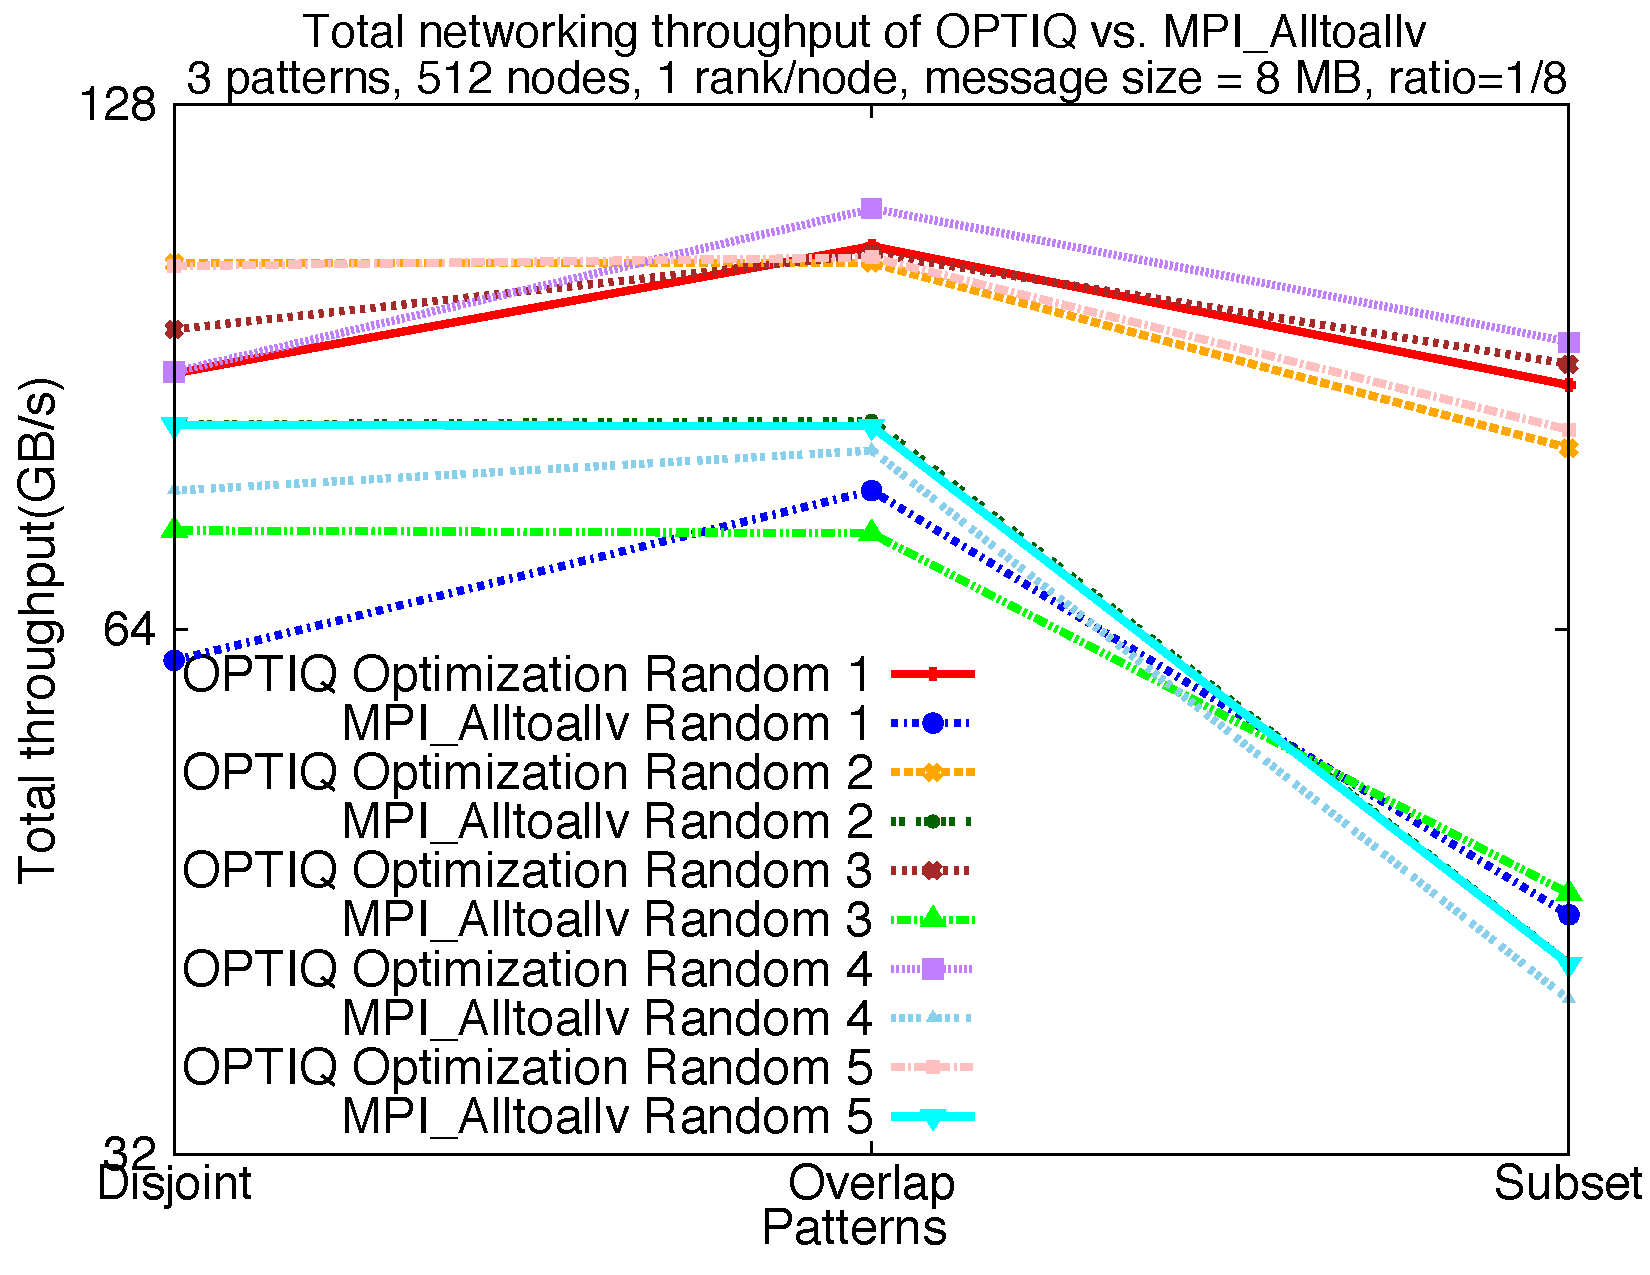
\includegraphics[scale=0.30]{figures/rand_opt_mpi.pdf}
\vspace{-0.1in}
\caption{Randomized sources and destination while keeping the same set of nodes}
\vspace{-0.1in}
\label{fig:random}
\end{figure}


\subsubsection{Constant the number of nodes p, sources m and destination n, vary the average distance d between sources and destinations}
This is to show that with longer distance, we have more paths to explore.

\begin{figure}[!htb]
\vspace{-0.1in}
\centering
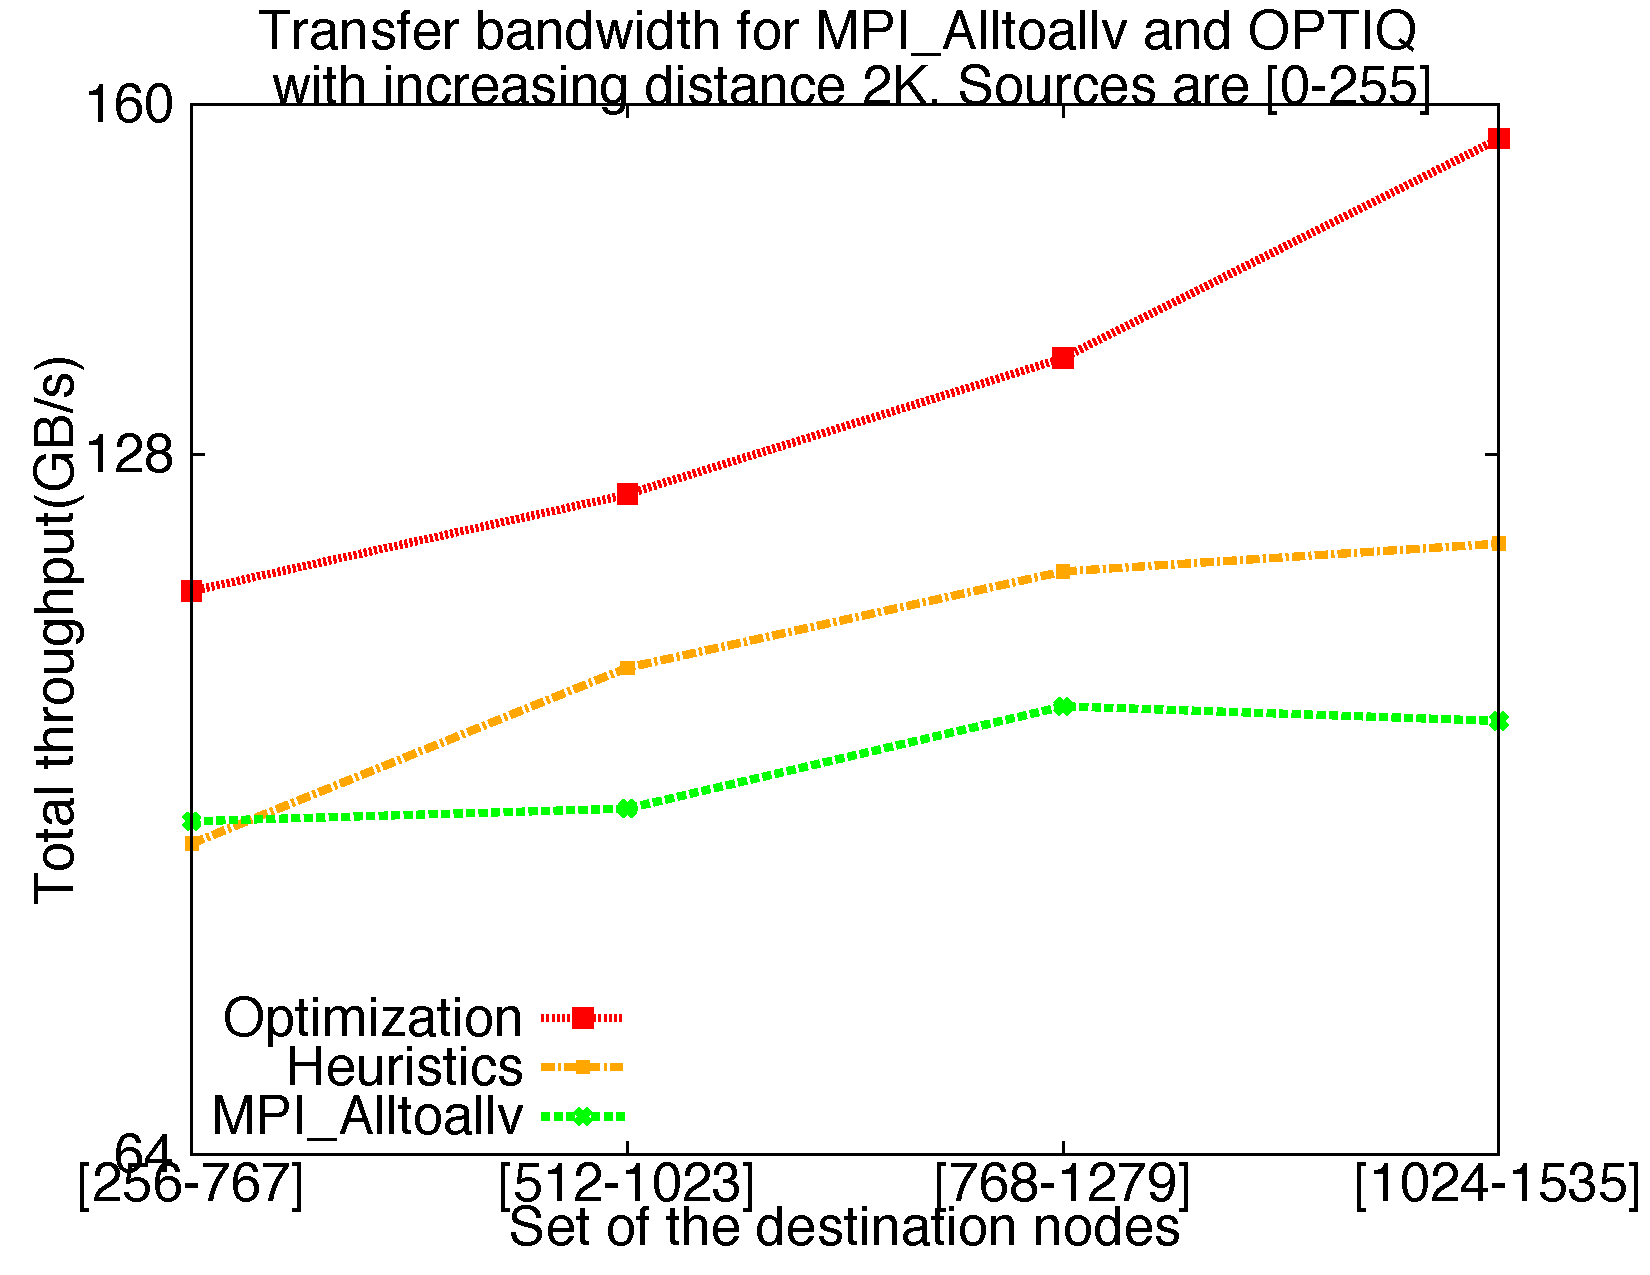
\includegraphics[scale=0.30]{figures/incrdist.pdf}
\vspace{-0.1in}
\caption{Total data movement throughput when increasing distance between sources and destinations}
\vspace{-0.1in}
\label{fig:incrdist}
\end{figure}

\subsubsection{Consant the number of node p and sources m, vary number of destinations n}
This is to show that with more number of destination, we have less paths to explore

\begin{figure}[!htb]
\vspace{-0.1in}
\centering
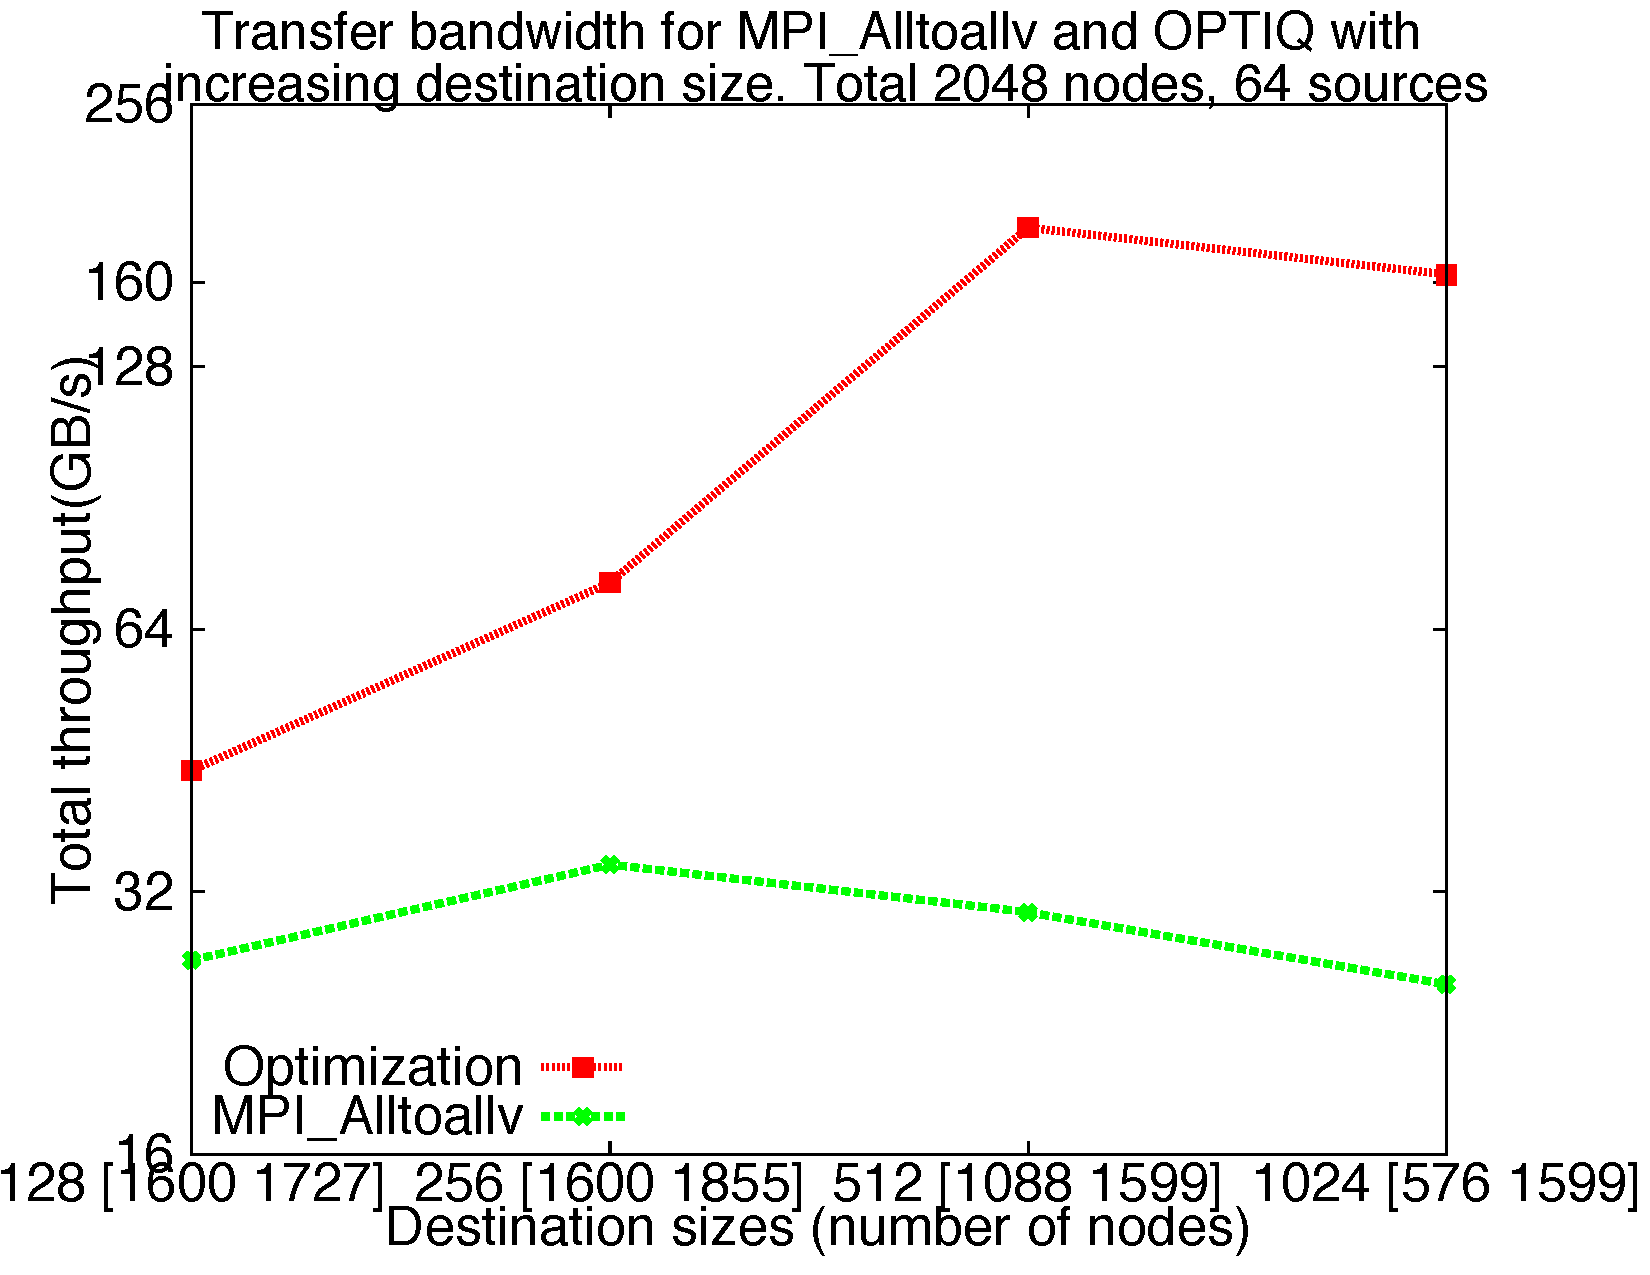
\includegraphics[scale=0.30]{figures/incrsize.pdf}
\vspace{-0.1in}
\caption{Total data movement throughput when increasing size of destinations}
\vspace{-0.1in}
\label{fig:incrsize}
\end{figure}

\subsubsection{Benchmark for chunk size}

To transfer dat through intermediate, we split a message into smaller chunks and keep sending the chunks into the network. It is to reduce the waiting time at the intermediate, thus, reduce the total transfer time. We do an experiment to see what is the optimal chunk size for each pattern. In this experiment, we generated 91 patterns (16 disjont patterns[expriment id 0-15], 48 overlap patterns [16-63], 27 subset patterns [64-90]), in which we vary the number of sources, destination and their locaiton in the 2048-node partition. We varied the chunk size from 8 KB to 1 MB to find the most optimal chunk size. However for the sake of simplicity, we only show the results of chunk sizes from 32 KB to 512 KB while not losing the accuracy of the experiment. The results are shown in Figure \ref{fig:chunksize}.

\begin{figure}[!htb]
\vspace{-0.1in}
\centering
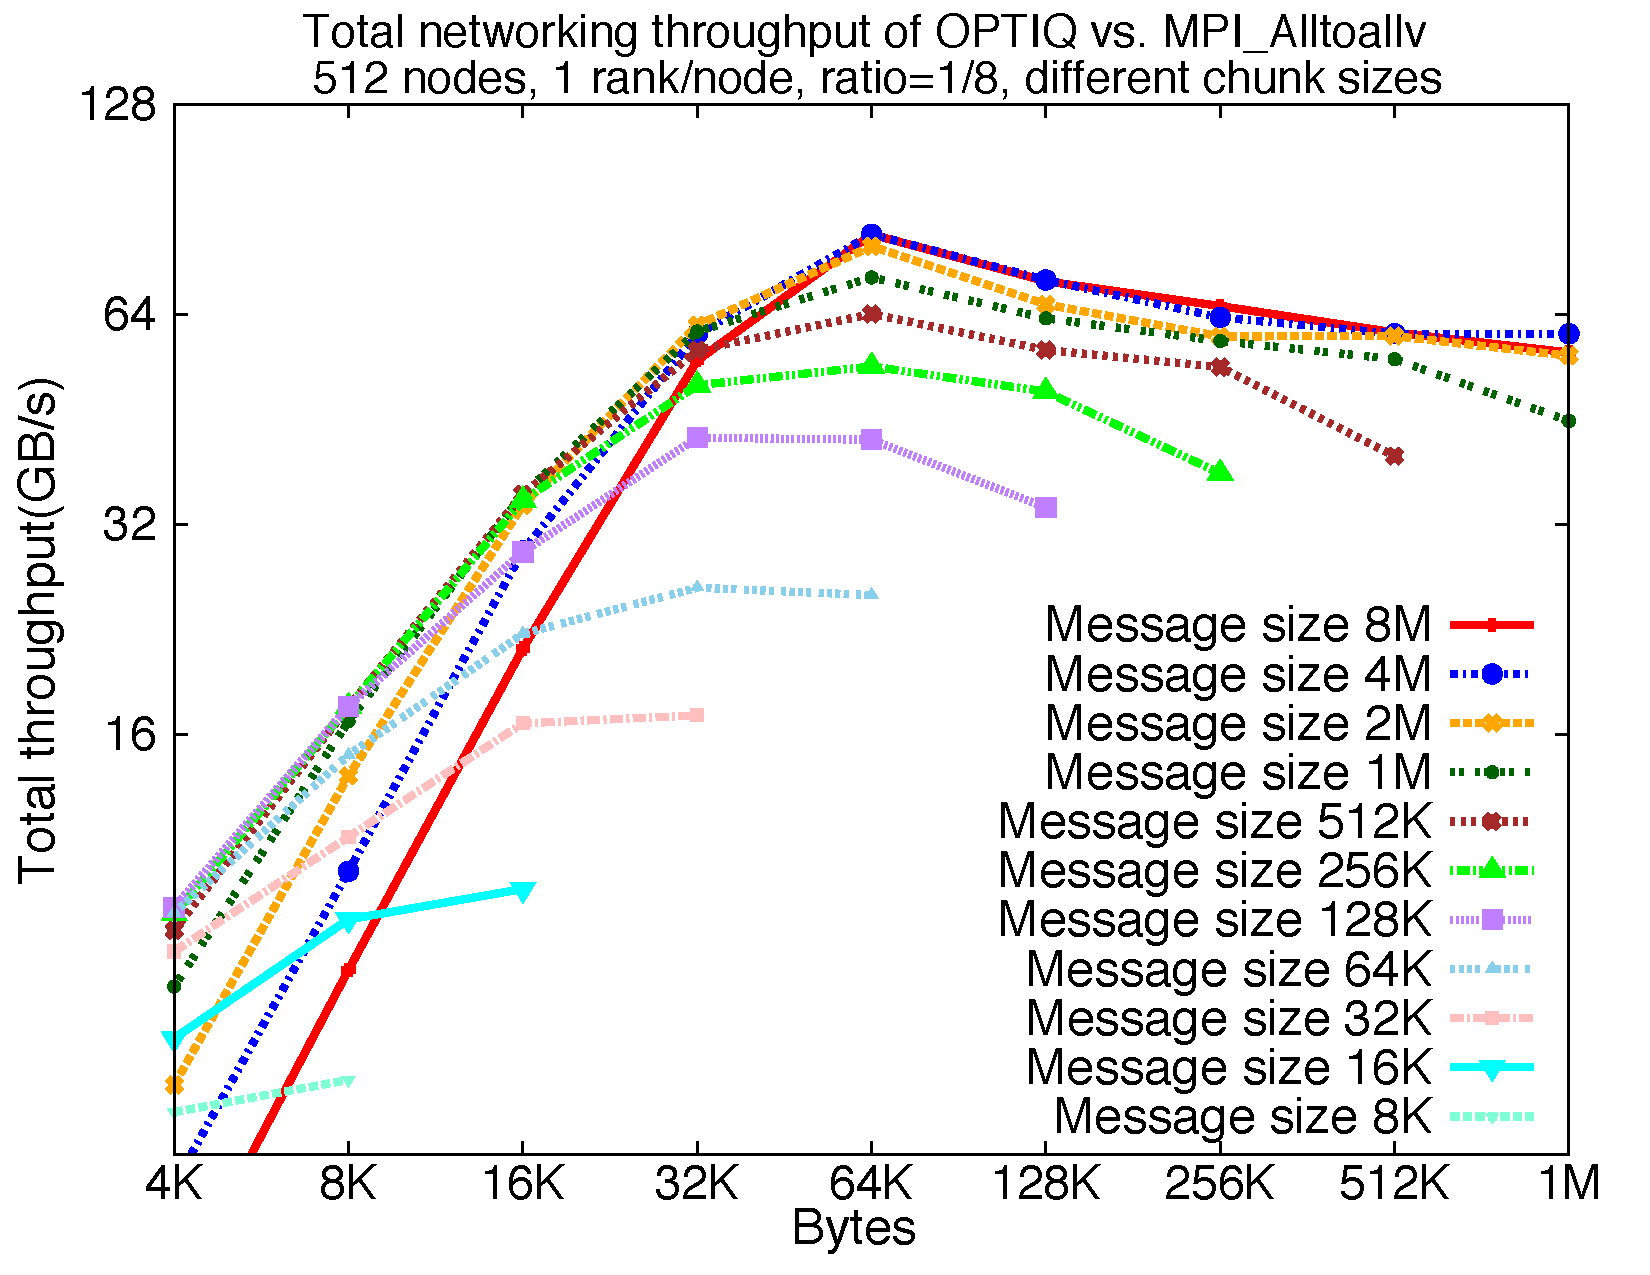
\includegraphics[scale=0.30]{figures/87_chunksize.pdf}
\vspace{-0.1in}
\caption{Chunk sizes and their performance in 512-node partition, subset pattern}
\vspace{-0.1in}
\label{fig:chunksize}
\end{figure}

We can see that, for disjoint and overlap patterns, most of the time the chunk size of 64 KB and/or 128 have dominated performance. For the subset patterns, chunk size 128 KB is clearly optimal choice. In order to be consistent, in the above experiments, we used 64 KB chunk size for disjoint and overlap pattern and 128 KB chunk size for subset patterns.

\subsubsection{Message size scaling}

\begin{figure}[!htb]
\vspace{-0.1in}
\centering
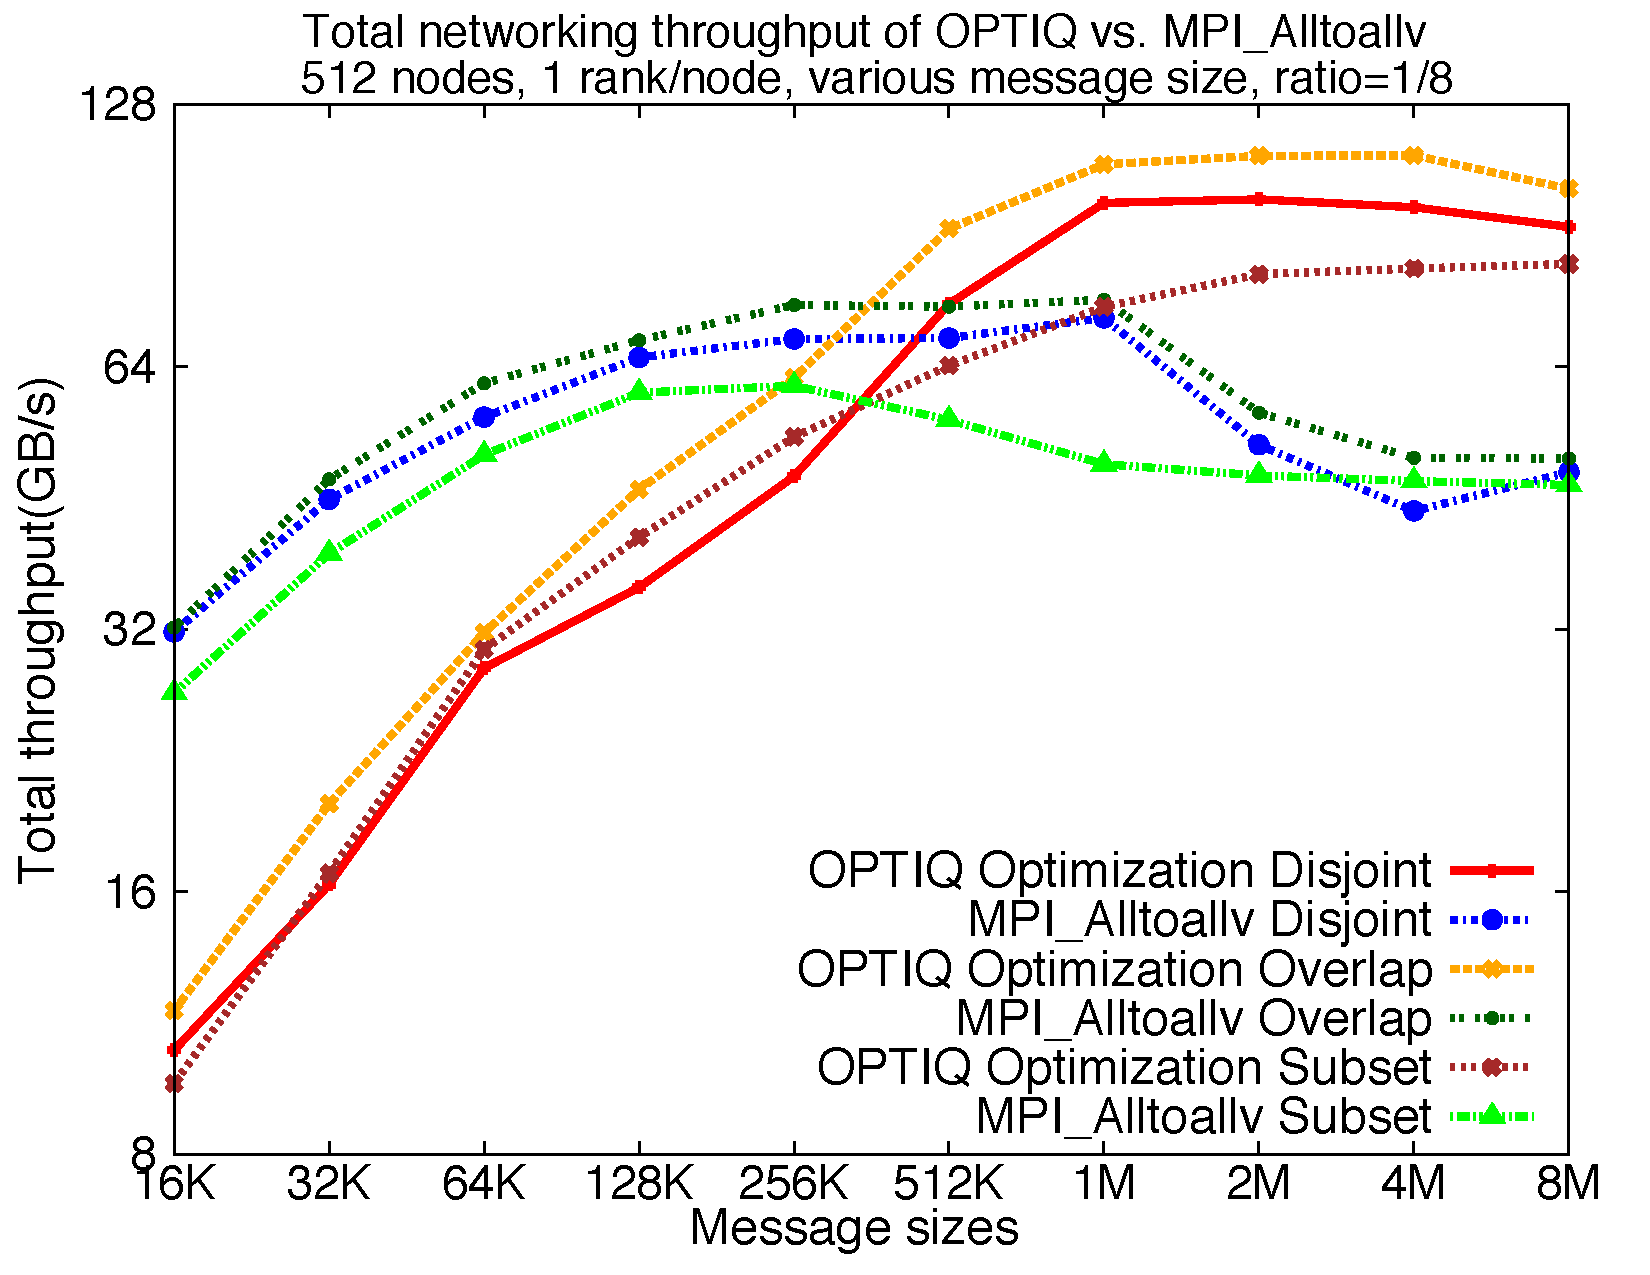
\includegraphics[scale=0.30]{figures/messagesize.pdf}
\vspace{-0.1in}
\caption{Total throughtput with different message sizes in 3 patterns}
\vspace{-0.1in}
\label{fig:messagesize}
\end{figure}

\subsubsection{Number of paths fed into heuristics II}

Quality i.e the performance based on the number of paths

\begin{figure}[!htb]
\vspace{-0.1in}
\centering
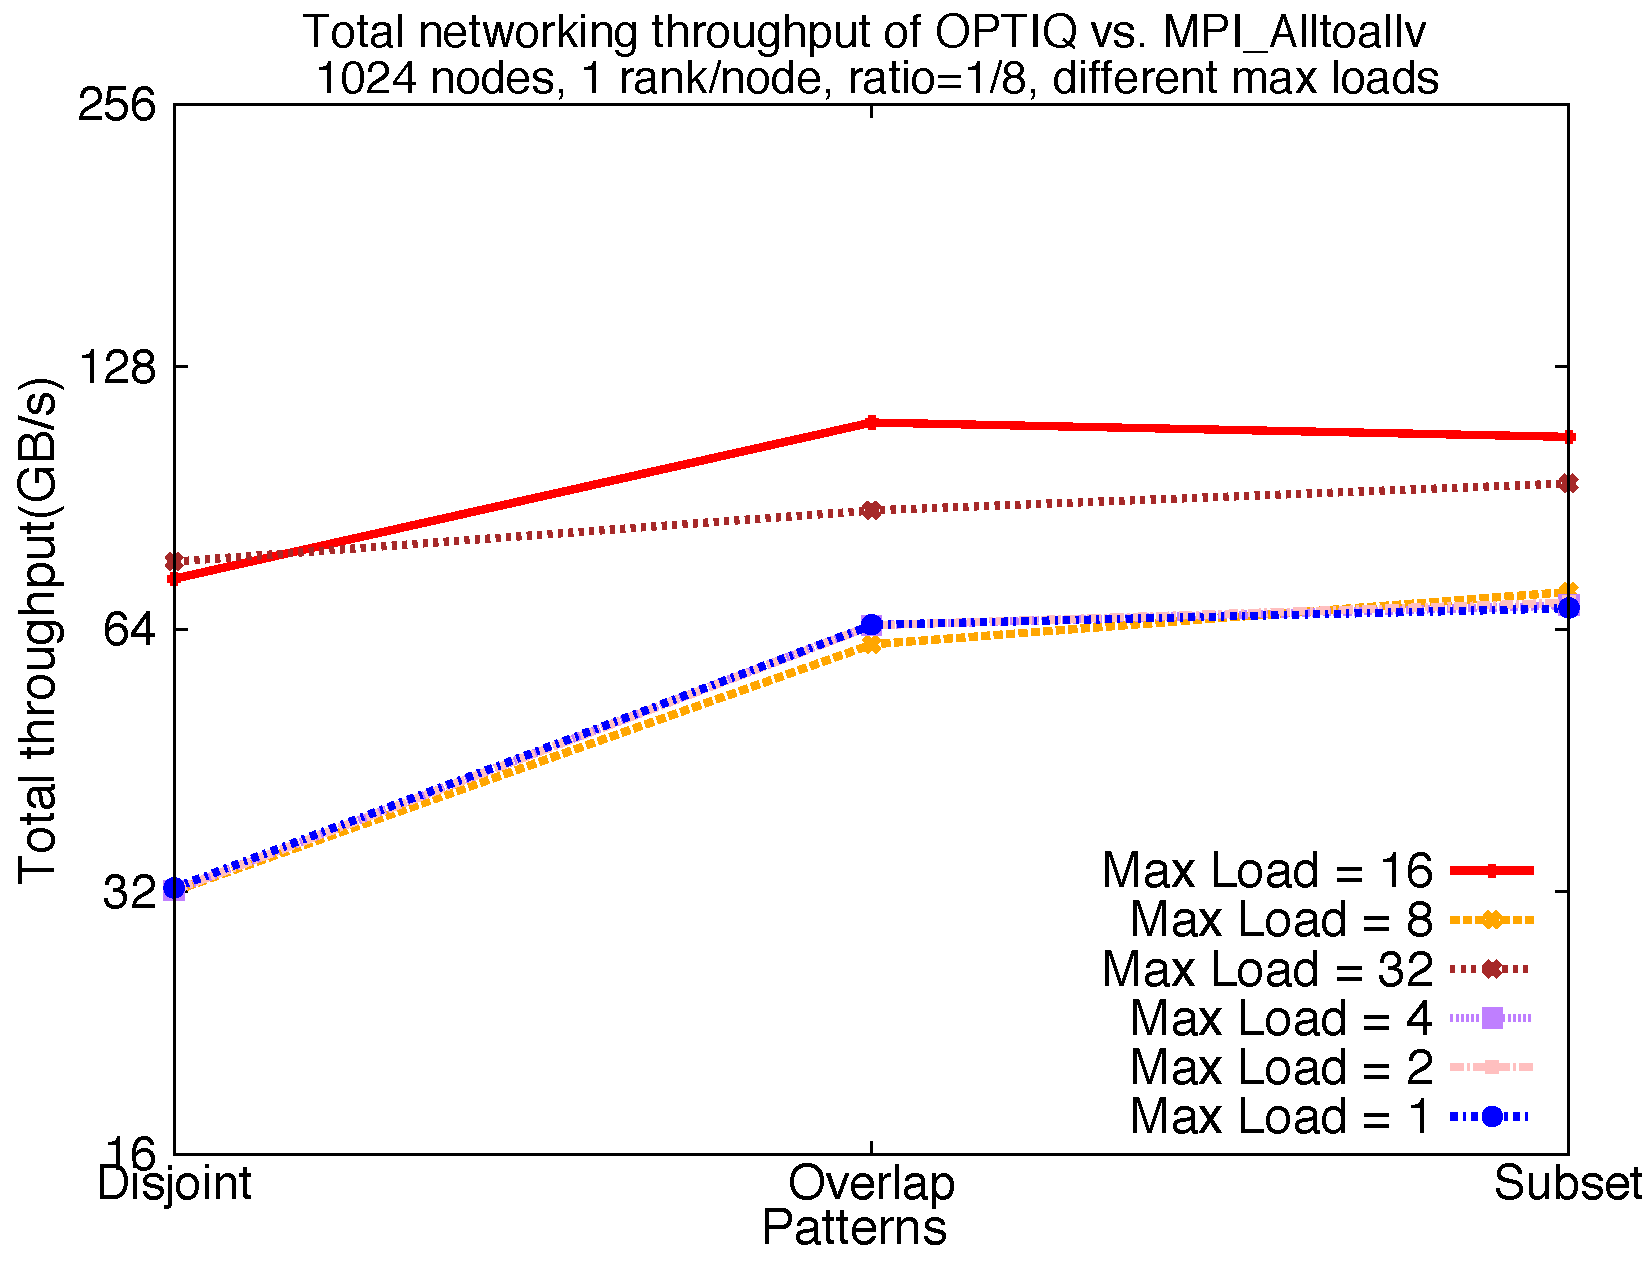
\includegraphics[scale=0.30]{figures/heu_paths_3p.pdf}
\vspace{-0.1in}
\caption{Different number of maxload}
\vspace{-0.1in}
\label{fig:heu_paths_3p}
\end{figure}

Time to search for paths

\begin{table}[!htbp]
   \centering
   \begin{tabular}{| p {0.75cm}| r | r | r | r | r | r |}
    \hline
    \multirow{2}{*}{Pattern} & \multicolumn{6}{ c| }{Time for Different Max Load (s)} \\ \cline{2-7}
    & 1 & 2 & 4 & 8 & 16 & 32 \\ \hline
    Disjoint & 1.958 & 1.961 & 1.917 & 1.956 & 2.002 &  2.164 \\ \hline
    Overlap & 1.923 & 1.890 & 1.801 & 1.929 & 1.993 & 2.082 \\ \hline
    Subset & 1.907 & 1.870 & 1.891 & 1.955 & 2.024 &  2.223 \\ \hline
    \end{tabular}
    \caption{Search time with diffent max load in 1024 nodes partition}
    \label{table:solvetime}
\end{table}

\subsubsection{Number of paths fed into model}

Quality

\begin{figure}[!htb]
\vspace{-0.1in}
\centering
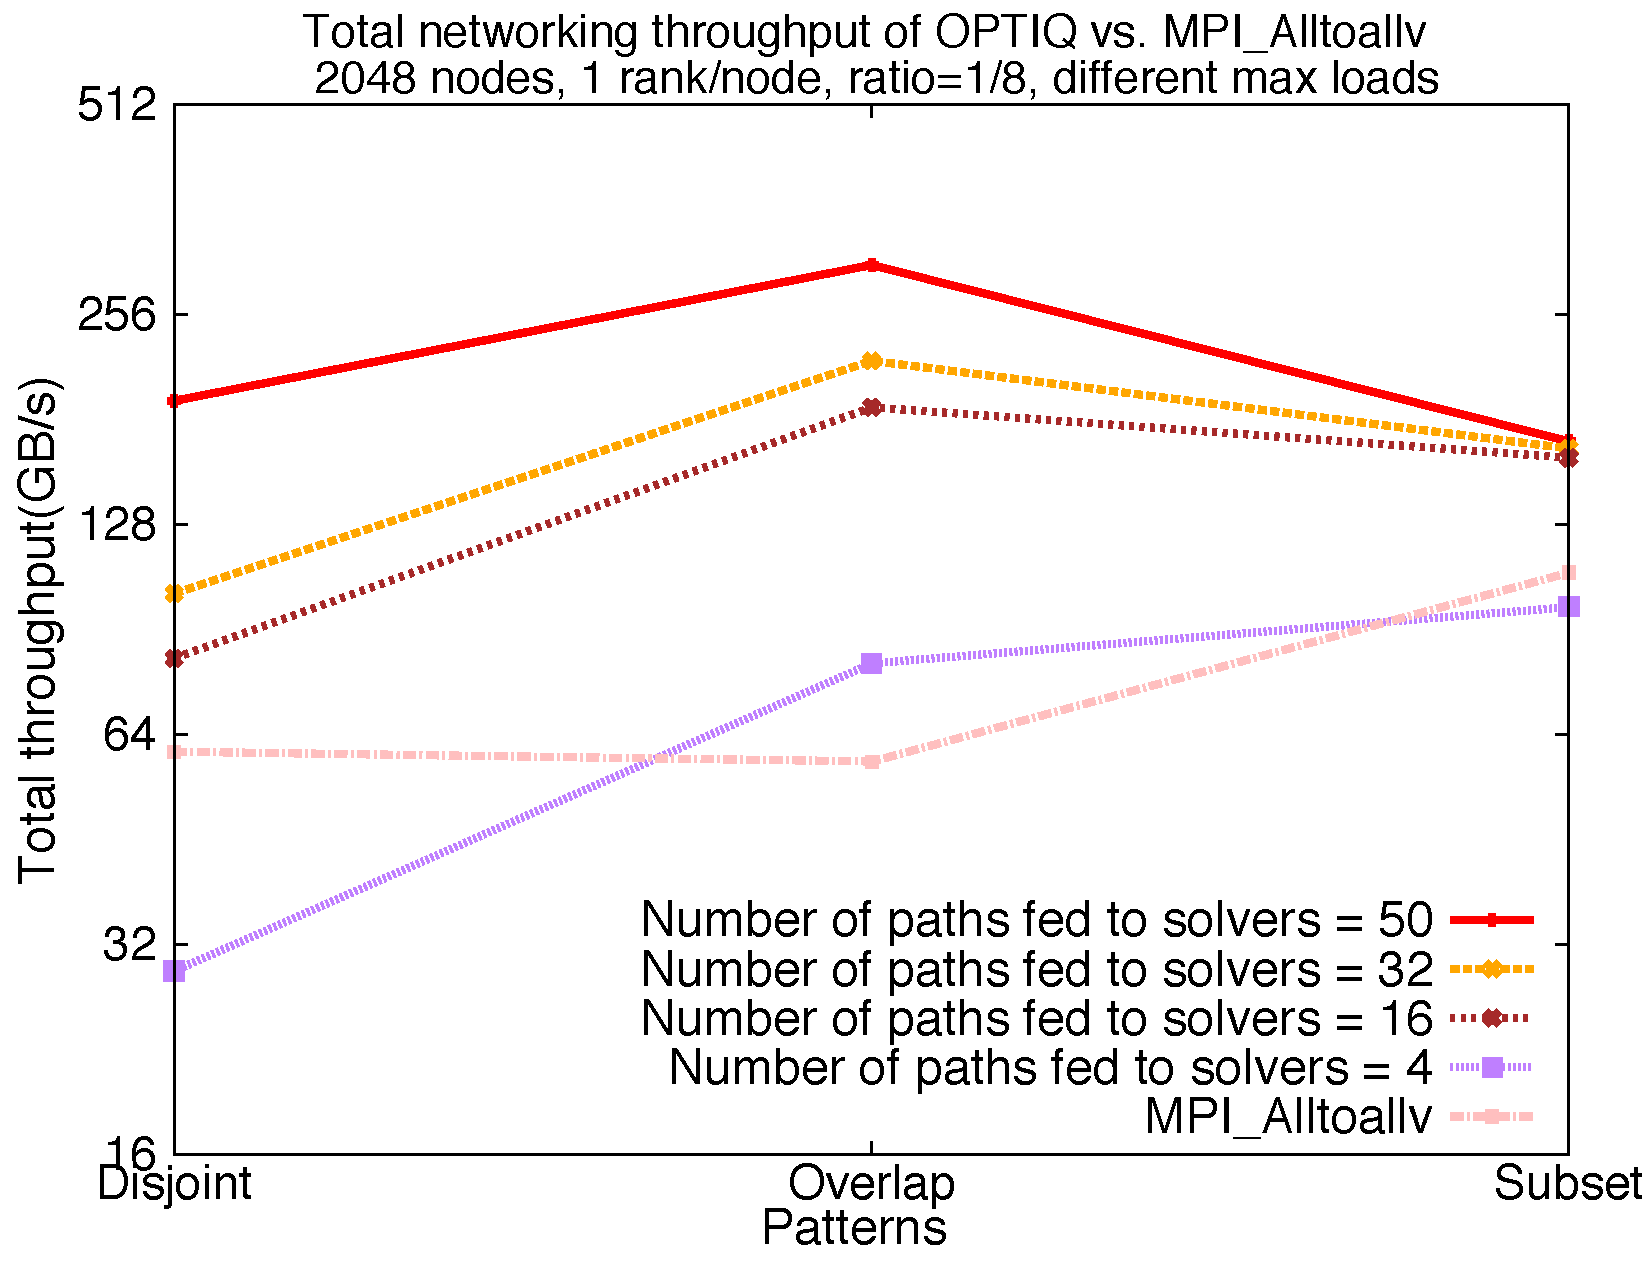
\includegraphics[scale=0.30]{figures/opt_paths_3p.pdf}
\vspace{-0.1in}
\caption{Total throughput with different number of paths fed into solvers}
\vspace{-0.1in}
\label{fig:opt_paths_3p}
\end{figure}

Time to search for paths

\begin{table}[!htbp]
   \centering
   \begin{tabular}{| p {0.75cm}| p{0.5cm} | r | p{0.5cm} | p{0.5cm} | r | r | r | r |}
    \hline
    \multirow{2}{*}{Pattern} & \multicolumn{4}{ c| }{AMLP time (s)} & \multicolumn{4}{ c| }{Solve time (s)} \\ \cline{2-9}
    & 4 & 16 & 32 & 50 & 4 & 16 & 32 & 50 \\ \hline
    Disjoint & 13.9 & 187.7 & 123.0 & 224.0 & 0.06 & 6.6 & 4.4 & 84.0 \\ \hline
    Overlap & 13.6 & 51.9 & 134.6 & 198.7 & 0.09 & 16.6 & 179.4 & 530.3 \\ \hline
    Subset & 14.4 & 50.6 & 134.9 & 217.3 & 0.85 & 111.3 & 173.2 & 939.6 \\ \hline
    \end{tabular}
    \caption{AMPL and solving time}
    \label{table:solvetime}
\end{table}

\begin{comment}
\subsubsection{Subset - Type 2 (Subgroup Data Aggregation)}

In the subgroup data aggregation experiment, we aggregated data within a subgroup to one node in the subgroup. In this experiment, we used a 512-nodes partition. The partition was divided into subgroup of size 4, 8, 16, 32, and 64 nodes each. One node in the middle of a subgroup was selected as the destination to aggregate data from all nodes in the subgroup(including itself). The data size is 1MB. We aggregate data using MPI\_Alltoallv and our framework for 20 times, measured and reported the average of the measurements. The aggregation bandwidths are shown in Figure \ref{fig:aggbw}.

\begin{figure}[!htb]
\vspace{-0.1in}
\centering
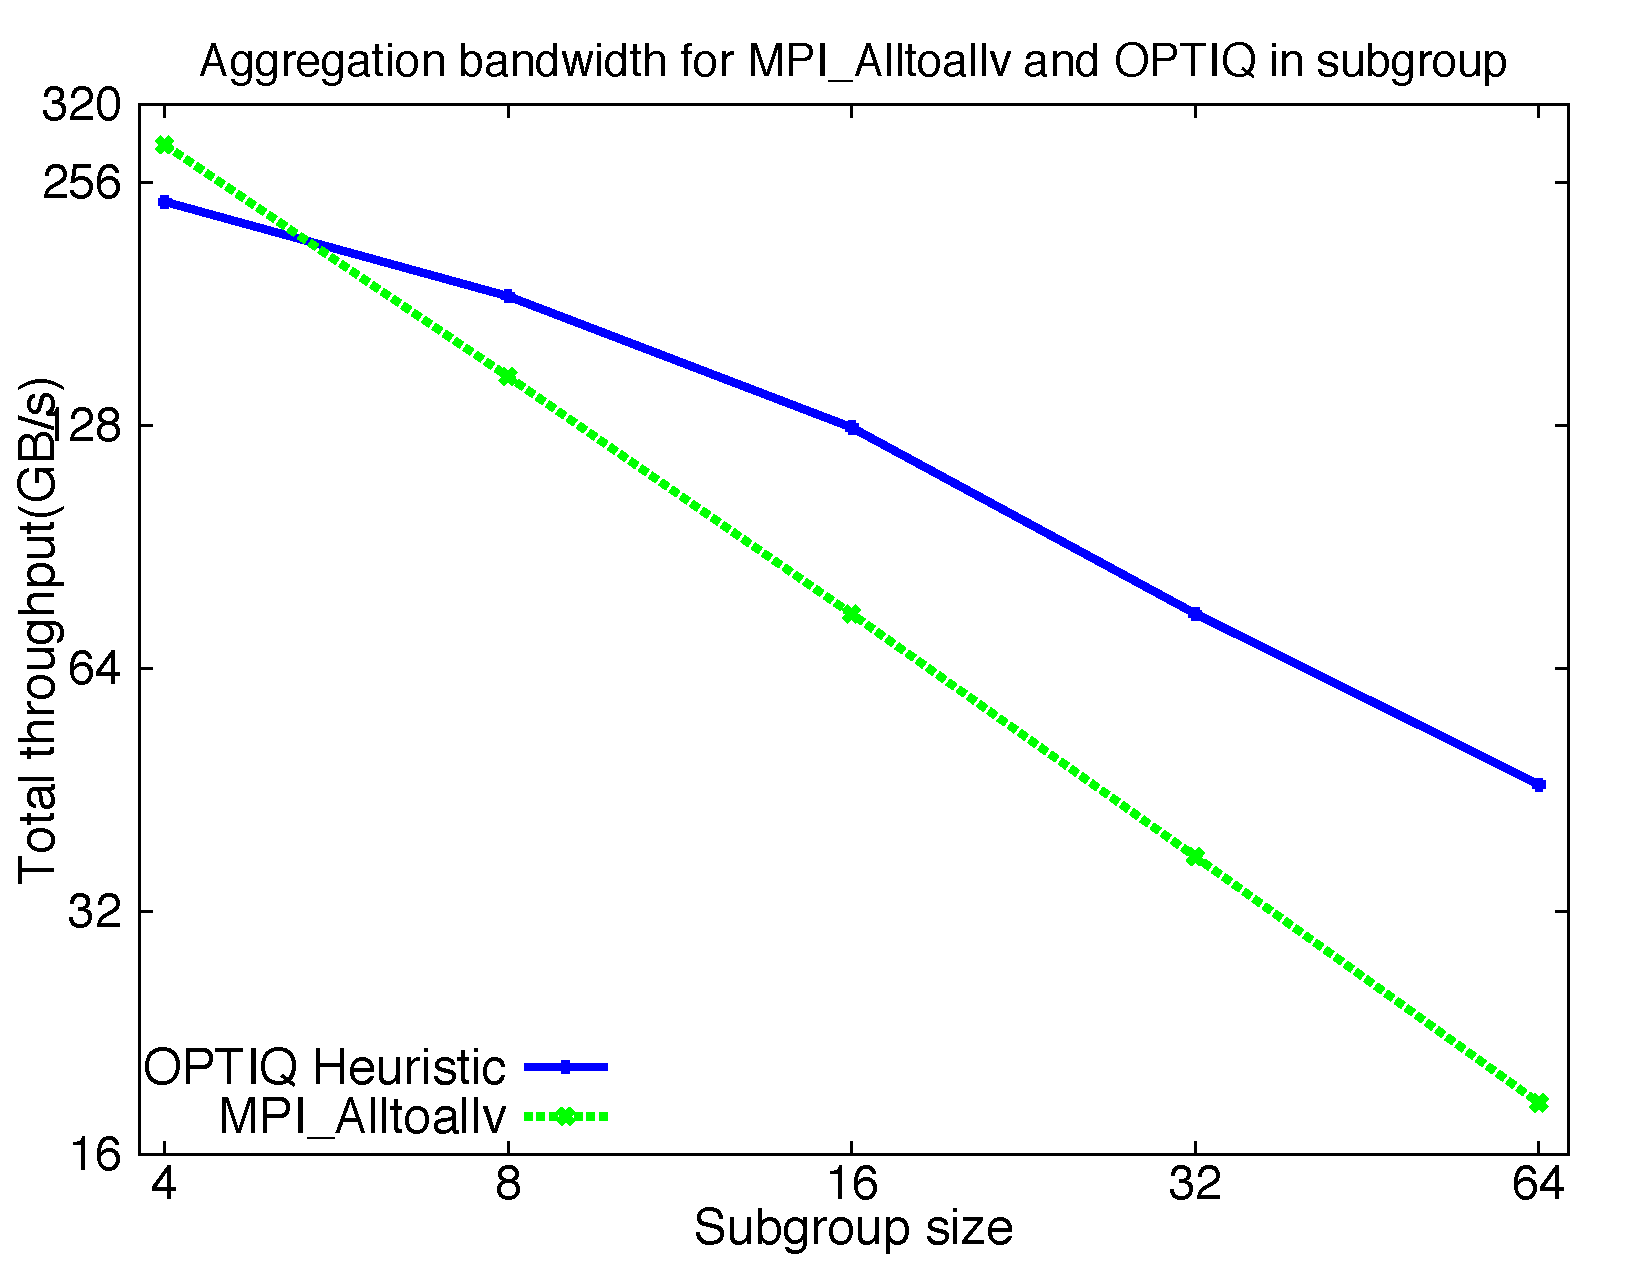
\includegraphics[scale=0.30]{figures/agg.pdf}
\vspace{-0.1in}
\caption{Aggregation bandwidth}
\vspace{-0.1in}
\label{fig:aggbw}
\end{figure}

As we can see in the figure, our work shows better performance as we increased subgroup size due to more balanced networking load. At the beginning when teh size of subgroups is 4, MPI\_Alltoallv performed better. But as we doubled the subgroup size OPTIQ started to get better i.e. 1.25X at 8 nodes/subgroup, 1.7X at 16 nodes/subgroup, 2X at 32 nodes/subgroup and 2.5X at 64 nodes/subgroup. This is because OPTIQ has better network load balancing. We show the network load in the Figure \ref{fig:aggload}

\begin{figure}[!htb]
\vspace{-0.1in}
\centering
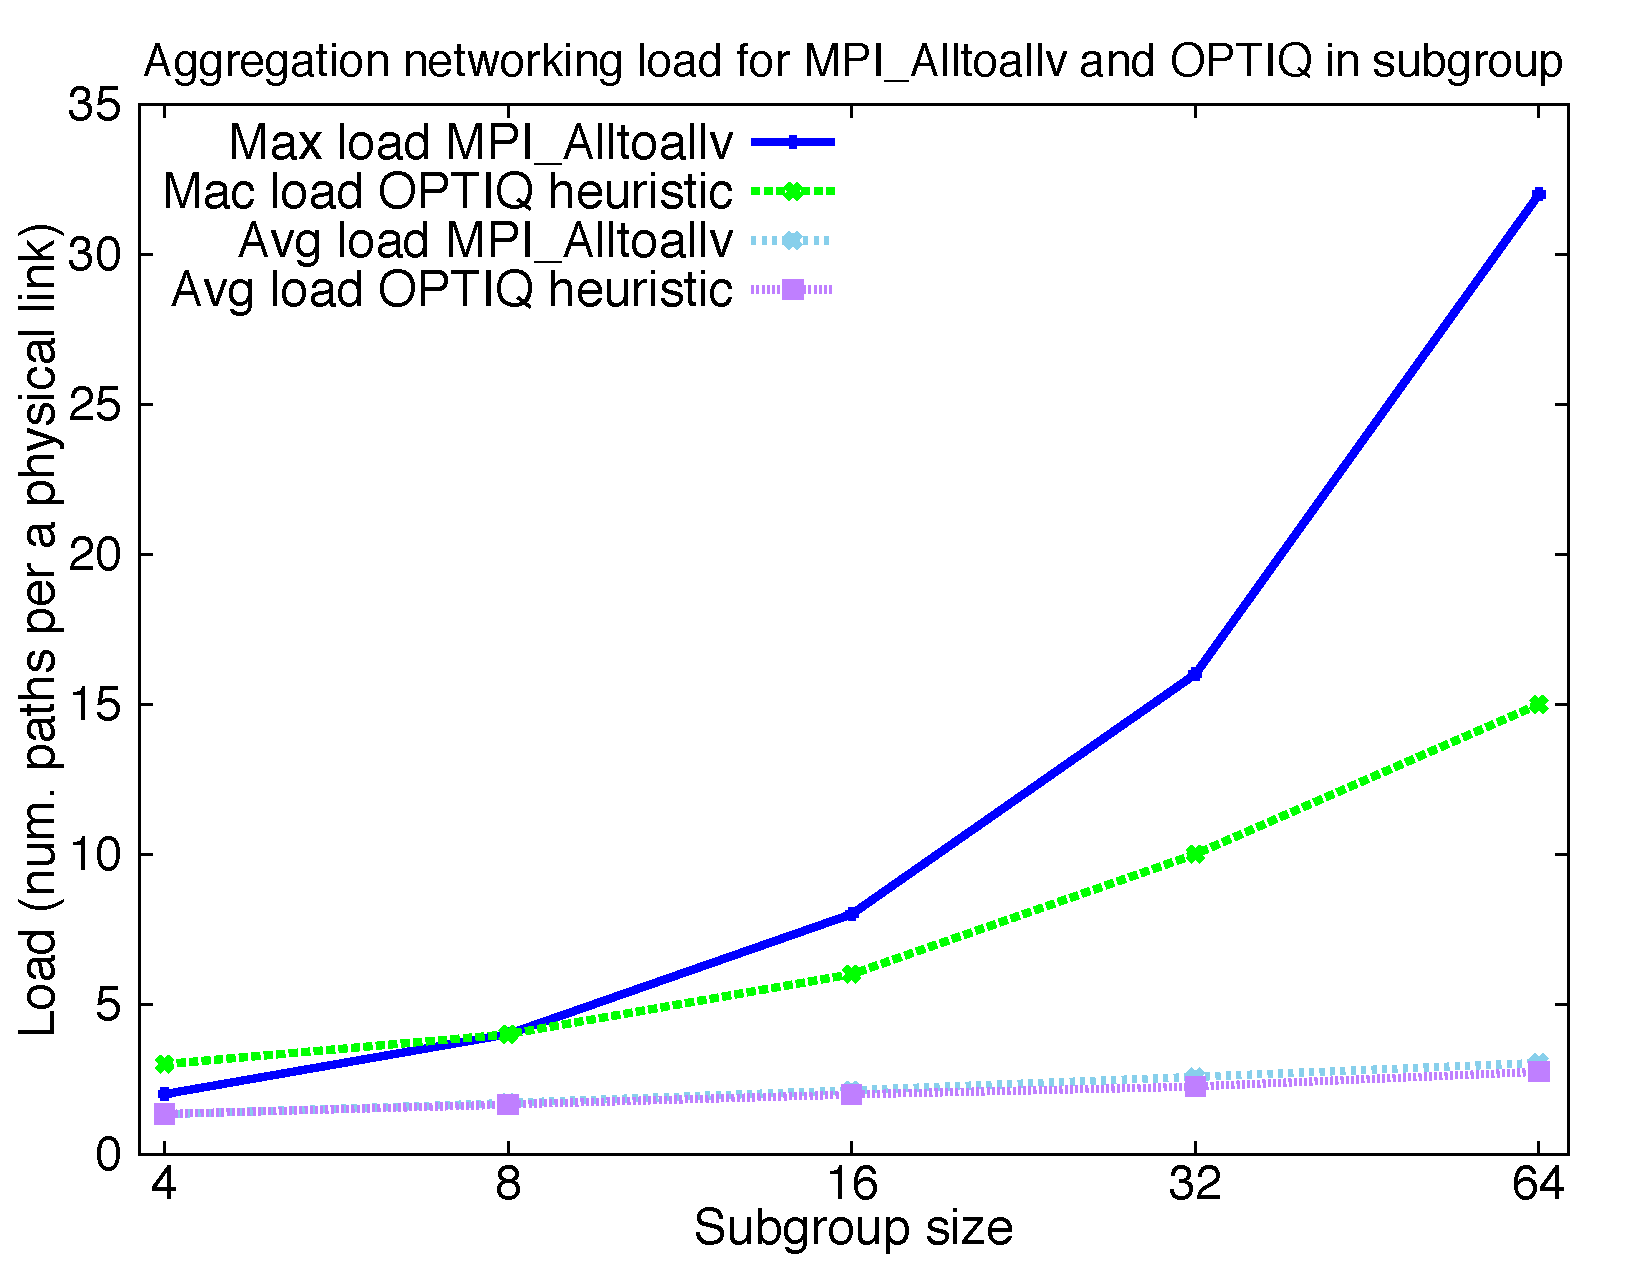
\includegraphics[scale=0.30]{figures/load.pdf}
\vspace{-0.1in}
\caption{Networking load over links}
\vspace{-0.1in}
\label{fig:aggload}
\end{figure}

Figure \ref{fig:aggload} shows the max and average loads for both MPI\_Alltoallv and OPTIQ. Load is number of paths that used a physical link. As we can see in the figure, when the group size increased the average load is approximate the same, but max load increased much faster in MPI\_Alltoallv compare to OPTiQ. This is because MPI\_Alltoallv used default routing algorithm. The default routing algorithm routes data in the longest dimension first leading to more load on certain links and no loads on many other links. Hence the max load in MPI\_Alltoalllv is higher than OPTIQ. Our work distributes the networking load over more links with lower max load. The networking distribution is shown in Figure \ref{fig:aggdist}

\begin{figure}[!htb]
\vspace{-0.1in}
\centering
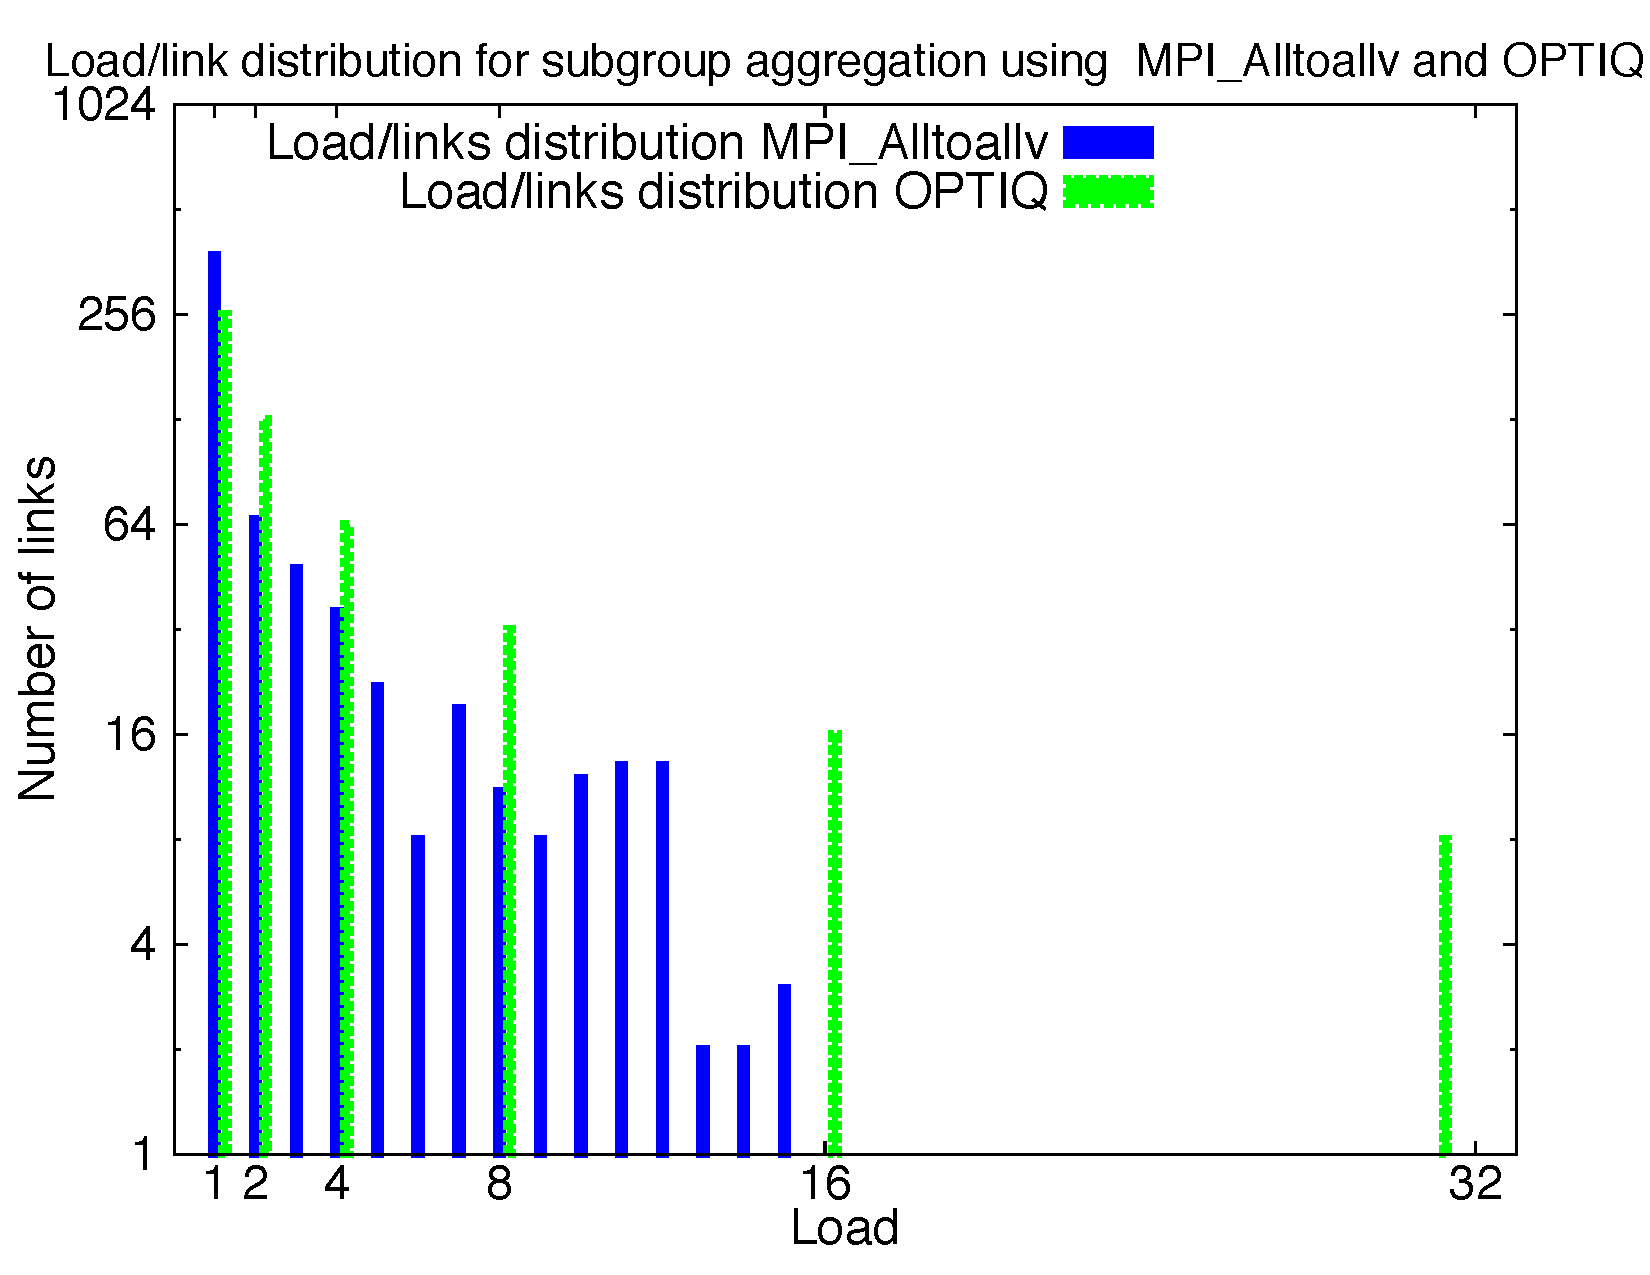
\includegraphics[scale=0.30]{figures/distribution.pdf}
\vspace{-0.1in}
\caption{Networking load disitribution over links}
\vspace{-0.1in}
\label{fig:aggdist}
\end{figure}

Figure \ref{fig:aggdist} shows that our work has a better networking load distribution. All of the loaded links have max load at most of 15, with many links has low load. While MPI\_Alltoallv has 8 links with max load of 32. We achieved better load distribution by using more links and by using longer links. This leads to a litte higher max hops (1 or 2 hops) and average hops used. The Figure \ref{fig:agghop} shows the maximum and average nuber of hops used.

\begin{figure}[!htb]
\vspace{-0.1in}
\centering
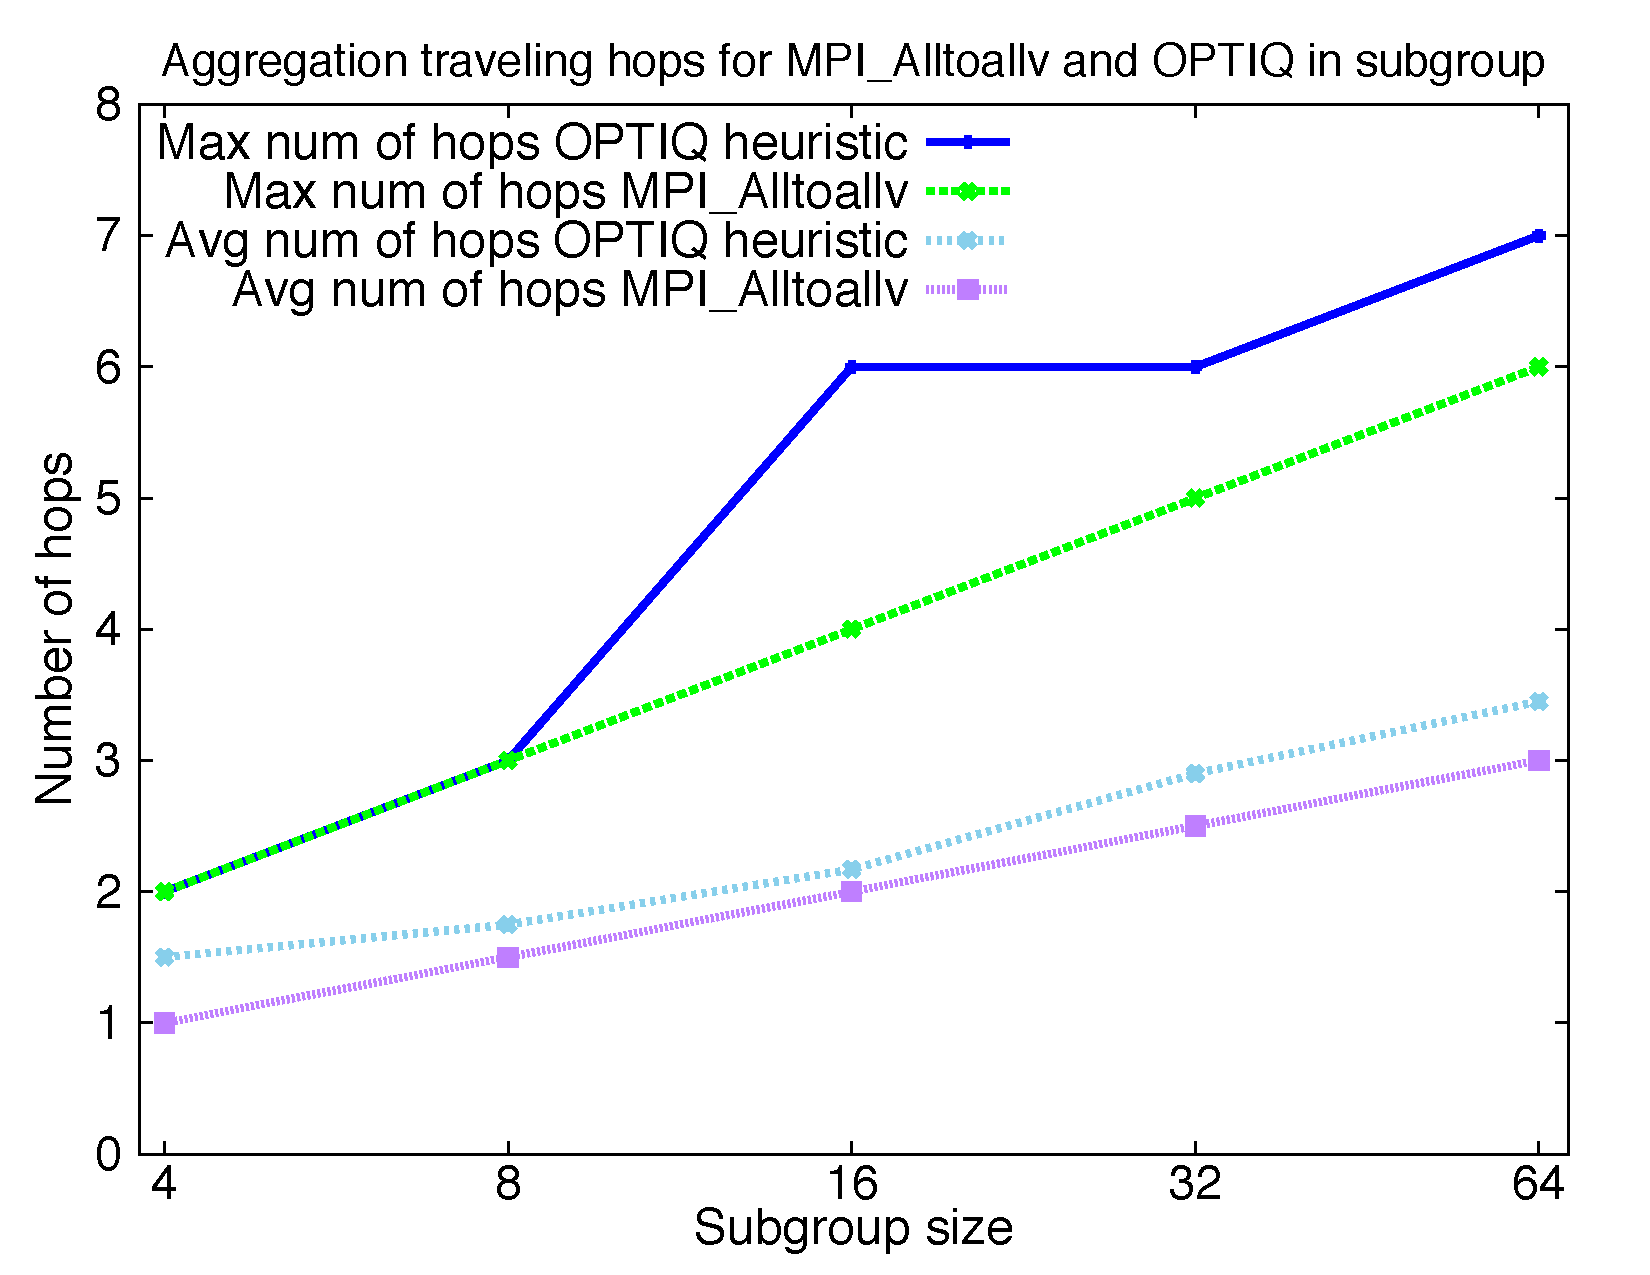
\includegraphics[scale=0.30]{figures/hop.pdf}
\vspace{-0.1in}
\caption{Max and average hops in data aggregation}
\vspace{-0.1in}
\label{fig:agghop}
\end{figure}

In the Figure \ref{fig:agghop} we can see that compare to MPI\_Alltoallv, OPTIQ used 1 to 2 hops more in case of maximum number of hops and 0.5 hops more in case of average number of hops. This is because OPTIQ explored longer paths to avoid increasing max load. The algorithms we have also try to balance between number of hops and max load as too long paths can actually increase time hence degrade data movement bandwidth.

\subsection{Scalability}
Show scalability by partition size, number of ranks per node and message sizes

\end{comment}
